\documentclass[12pt]{article}

\usepackage{sbc-template}
\usepackage{graphicx,url}
\usepackage[utf8]{inputenc}
\usepackage[brazil]{babel}

\usepackage{float}
\usepackage{mathtools}
     
\sloppy

\title{Instructions for Authors of SBC Conferences\\ Papers and Abstracts}

\author{Luiz Henrique Souza Caldas, Daniel Ratton Figueiredo} 


\address{Programa de Engenharia de Sistemas e Computação (PESC) \\ Instituto Alberto Luiz Coimbra de Pós-Graduação e Pesquisa de Engenharia (COPPE) \\ Universidade Federal do Rio de Janeiro (UFRJ)\\
  \email{lhscaldas@cos.ufrj.br, daniel@cos.ufrj.br}
}

\begin{document} 

\maketitle
     
\begin{resumo} 
  Este meta-artigo descreve o estilo a ser usado na confecção de artigos e
  resumos de artigos para publicação nos anais das conferências organizadas
  pela SBC. É solicitada a escrita de resumo e abstract apenas para os artigos
  escritos em português. Artigos em inglês deverão apresentar apenas abstract.
  Nos dois casos, o autor deve tomar cuidado para que o resumo (e o abstract)
  não ultrapassem 10 linhas cada, sendo que ambos devem estar na primeira
  página do artigo.
\end{resumo}

\section{Introdução}

O Brasil possui uma extensa costa de 8{,}7 mil quilômetros, com 68 portos e uma faixa litorânea que concentra mais da metade da população e do PIB do país. Além disso, o país possui aproximadamente 4{,}5 milhões de quilômetros quadrados de águas jurisdicionais, onde se encontram recursos estratégicos como 95\% do petróleo e 83\% do gás natural nacionais, e por onde transitam cerca de 95\% do comércio exterior \cite{andrade_2021}.
Nesse contexto, a crescente adoção de Veículos Aéreos Não Tripulados (VANTs) em operações de vigilância marítima exige métodos mais robustos de planejamento de rotas, especialmente em cenários com alvos parcialmente conhecidos e detecção sensorial sujeita a limitações práticas. Trabalhos anteriores mostram que a vigilância baseada em varredura aérea pode ser modelada como uma variação do Problema do Caixeiro Viajante (TSP), incorporando restrições operacionais como autonomia limitada, sensores com alcances distintos e alvos móveis ou parcialmente observáveis \cite{marlow_2007}.
Técnicas de otimização como o \textit{Simulated Annealing} têm se mostrado eficazes em problemas de roteamento com grande espaço de busca e múltiplos mínimos locais, sendo uma escolha promissora para o replanejamento progressivo de trajetos em ambientes com inserção dinâmica de alvos \cite{kosmas_2012}.
Mais recentemente, abordagens com replanejamento dinâmico em tempo real vêm sendo propostas para garantir a cobertura de alvos não detectados ou mal inspecionados, especialmente em aplicações com VANTs e sensores embarcados \cite{penicka_2017}. Motivado por esses avanços, este trabalho propõe uma formulação adaptada do TSP para missões de patrulha marítima com inserção condicional de novos alvos, levando em conta restrições de distância lateral, autonomia do VANT e alcance heterogêneo de sensores.

\begin{figure}[H]
    \centering
    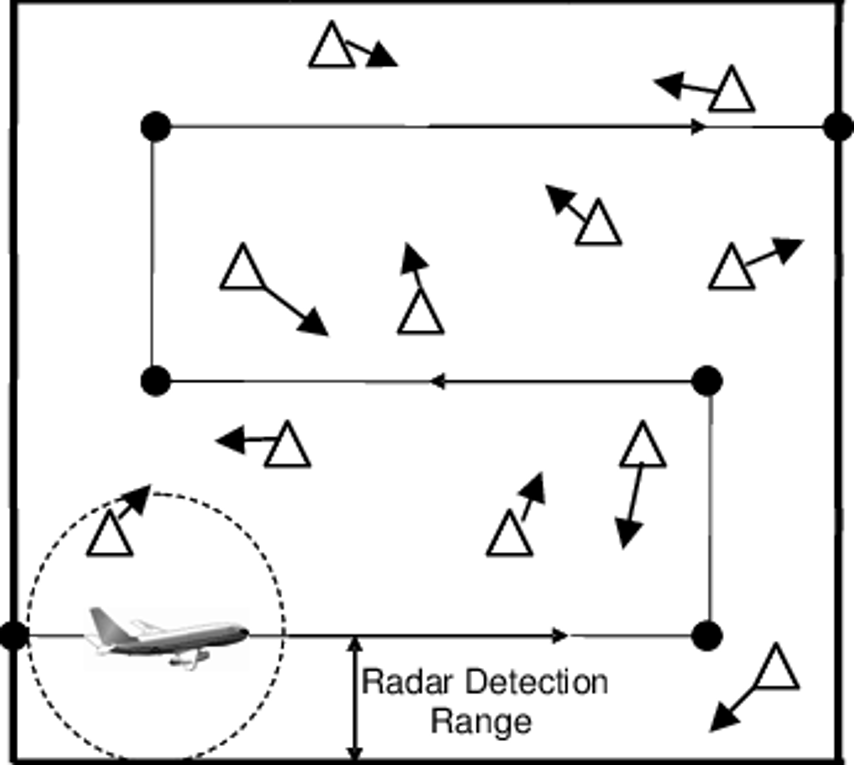
\includegraphics[width=0.5\textwidth]{fig/vant.png}
    \caption{Patrulha naval realizada por aeronave.}

    \small
    \textbf{Fonte:} Marlow et al 2007 \cite{marlow_2007}.
 \end{figure}
\section{Objetivo}
O objetivo deste trabalho é desenvolver uma metodologia para o planejamento dinâmico de rotas de VANTs em missões de vigilância marítima, considerando a detecção progressiva de alvos ao longo do percurso. A proposta visa adaptar o Problema do Caixeiro Viajante (TSP) a um contexto em que novos pontos de interesse são identificados durante a missão, e a decisão de incluí-los no trajeto deve considerar restrições operacionais e de sensoriamento. A solução deve permitir o replanejamento eficiente da rota, de forma a maximizar a inspeção de alvos relevantes, respeitando os limites de autonomia da aeronave.
\section{Metodologia}

A abordagem proposta consiste em simular missões de vigilância marítima utilizando Veículos Aéreos Não Tripulados (VANTs), os quais percorrem uma rota pré-definida composta por linhas paralelas. Essa rota representa um padrão sistemático de patrulhamento e é gerada automaticamente com base em parâmetros como ponto inicial, largura da área, espaçamento entre linhas e número de passagens.

Durante o voo, o VANT está equipado com dois sensores: um radar, responsável por detectar navios dentro de um raio de ação (50 milhas náuticas), e uma câmera de inspeção visual com alcance menor (20 milhas náuticas), utilizada para confirmar a identificação de alvos. Quando um navio entra na zona de alcance do radar, seu estado é atualizado para ``detectado''. Caso venha a entrar na área de alcance da câmera, ele é considerado ``inspecionado''.

O VANT atualiza sua lista de destinos a serem visitados com base em diferentes políticas de decisão:

\begin{itemize}
    \item \textbf{Política passiva}: o VANT mantém sua rota original, ignorando completamente os alvos detectados e identificando apenas os navios que a câmera alcança sem que ele desvie da trajetória planejada.

    \item \textbf{Política \textit{greed}}: os navios detectados e os waypoints ainda não percorridos da rota original são considerados simultaneamente, sendo reordenados com base na distância em relação à posição atual do VANT, priorizando os mais próximos em cada instante.
    \item \textbf{Política \textit{simulated annealing}}: os navios detectados e os waypoints ainda não percorridos da rota original também são considerados simultaneamente, mas utilizando uma técnica de amostragem estocástica baseada em \textit{Markov Chain Monte Carlo (MCMC)}. A lógica do algoritmo se baseia em uma cadeia de Markov com distribuição estacionária proporcional a uma função de Boltzmann, permitindo explorar o espaço de permutações de forma mais ampla, em busca de uma sequência globalmente mais eficiente em termos de distância percorrida.
\end{itemize}

O algoritmo de \textit{Simulated Annealing} implementado parte de uma solução inicial aleatória, composta pela lista de navios detectados e waypoints restantes, obtida por uma permutação aleatória desses pontos. O objetivo é encontrar a melhor ordem de visita, minimizando a distância total percorrida pelo VANT a partir de sua posição atual. A cada iteração, uma nova solução vizinha é gerada invertendo a ordem dos pontos em um subintervalo aleatório da rota atual. Essa operação de vizinhança é simples, mas suficientemente expressiva para explorar o espaço de soluções e escapar de mínimos locais.

Esse espaço de soluções pode ser interpretado como um grafo em que cada vértice representa uma permutação possível dos pontos a visitar, e as arestas conectam permutações que diferem por uma única inversão de subsegmento. Esse grafo é conexo e possui transições simétricas, o que garante que todas as soluções podem ser eventualmente alcançadas a partir de qualquer configuração inicial.

A nova solução é aceita com probabilidade 1 se sua distância total $f(s')$ for menor que a da rota atual $f(s)$, onde $s$ é a rota atual e $s'$ a rota vizinha gerada, e $f(s)$ denota a distância total percorrida ao seguir a rota $s$. Caso contrário, a nova rota ainda pode ser aceita com probabilidade $e^{-\frac{f(s') - f(s)}{T}}$, onde $T$ é um parâmetro chamado temperatura, que vai decaindo ao longo do processo. Essa estratégia permite aceitar, no início da execução, soluções piores de forma controlada, favorecendo a diversidade de caminhos explorados e contribuindo para escapar de mínimos locais.

A temperatura $T$ é atualizada ao longo do processo por meio de uma estratégia de resfriamento exponencial, seguindo a equação $T = T_0 \cdot \beta^t$, onde $T_0$ é a temperatura inicial, $\beta$ é um fator de decaimento ($0 < \beta < 1$), e $t$ representa a etapa atual. Em cada nível de temperatura, o algoritmo realiza um número fixo $N$ de perturbações da rota. Ao longo do processo, a melhor rota encontrada e seu respectivo custo são salvos sempre que superam o melhor valor anterior. Assim, ao final da execução, o algoritmo retorna a melhor sequência observada durante toda a busca, e não necessariamente a última solução gerada.

Apesar de sua flexibilidade, o algoritmo de \textit{Simulated Annealing} não está livre de limitações. Em particular, se a temperatura for reduzida rapidamente demais ao longo da execução, o processo pode ficar preso em mínimos locais, impedindo a descoberta de soluções mais eficientes. A escolha da estratégia de resfriamento adequada é, portanto, um fator crítico para o sucesso do método, sendo geralmente determinada por experimentação e ajuste fino para cada cenário.

Considera-se que os navios permanecem estáticos durante a simulação, dada a alta velocidade relativa do VANT em comparação às embarcações. O voo é interrompido automaticamente quando a autonomia total é atingida ou quando não há mais destinos a serem visitados. Os dados de desempenho como número de alvos detectados e inspecionados, distância percorrida e tempo de execução são registrados ao final da missão.






\bibliographystyle{sbc}
\bibliography{sbc-template}

\end{document}
